%\documentclass[final,3p]{article}
\documentclass[final,12p]{article}
\usepackage{graphicx}
\usepackage[letterpaper,margin=1.0in]{geometry}
\usepackage{amssymb}
\usepackage{changepage}
\usepackage{float}
\usepackage{hyperref}
\usepackage{url}
\usepackage{afterpage}
\usepackage{natbib}
\usepackage{setspace}
\usepackage{fancyhdr}
\pagestyle{fancy}
\fancyhf{}
\usepackage[utf8]{inputenc} 
\usepackage{lastpage}


\def\Student{Luis Enrique Cuevas  Picos}
\def\Title{THESIS PROJECT PROPOSAL}
\def\Prog{Doctorado en Ciencias (F\'{i}sica) }
\def\Dept{Departamento de Investigac\'{i}on en Fis\'{i}ca}
\def\Institution{Universidad de Sonora}
\def\Director{Dr. Jos\'{e} Feliciano Ben\'{i}tez Rubio}
\def\ProjectTitle{Luminosity measurement using Pixel Cluster Counting in the CMS experiment}
\def\ResearchLine{F\'{i}sica de Part\'{i}culas}

%%header and footer
\lhead{\Student\ / \Prog}
\rhead{\Title}
\rfoot{Page \thepage \hspace{1pt} of \pageref{LastPage}}


%%%%%%%comands
\newcommand{\SubItem}[1]{ {\setlength\itemindent{15pt} \item[-] #1} }
\newcommand{\lumi}[1]{{#1~fb$^{-1}$}}
\newcommand{\instlumi}[1]{#1$\times 10^{34}$ cm$^{-2}$s$^{-1}$}
  

%%%%%%%%%%%%%%%%%%%%%%%%%%%%%%%%%%%%%
\begin{document}
\onehalfspacing

%%%%Title Page
\begin{titlepage}
\centering
\hspace{0pt}
\vfill
{\scshape\Large \Title \par}
%project revised 2023-2
  
  \vspace{2cm}
  {
    TITLE:\par
    {\bf \large \ProjectTitle \par}
  }
       
  \vspace{0.5cm}
  {
    RESEARCH LINE: \par
    \ResearchLine \par
  }
        
  \vspace{4cm}
  {\underline{\hspace{8cm}}\par}
  {\bf \scshape \Student \par}
  {Student\par}

  \vspace{1cm}
  {\underline{\hspace{8cm}}\par}
  {\scshape \Director \par}
  {Director\par}

  \vspace{1cm}
  {\bf \Prog \par}
  {\Dept \par}
  {\Institution \par}

  \vspace{4cm}
  {\today}

\hspace{0pt}
\vfill

\end{titlepage}


%%%%% white page for print out
\shipout\null


%%%% Abstract Page
\newpage
\hspace{2pt}
\vfill

  \begin{center}
    {\Large \ProjectTitle \par}
    \vspace{1cm}
    {\itshape\textbf{Abstract}\par}
  \end{center}
  
  \vspace{0.5cm}
   
This research project proposes to enhance the precision of luminosity measurements at the LHC during Run 2 and Run 3, while also developing an upgraded luminosity measurement system for the HL-LHC phase. Accurate luminosity measurements are crucial for understanding particle physics, including Higgs boson production. The research involves analyzing the CMS pixel detector, calibrating it for 13.6 TeV collisions, and addressing systematic uncertainties. Additionally, it explores the Tracker Endcap
Pixel Detector's (TEPX) performance for HL-LHC conditions and develops new cluster counting algorithms. The project contributes to high-precision particle physics and will result in peer-reviewed publications and conference presentations.

  \hspace{2pt}
\vfill



%%%%%% Begin the body
\newpage
\section{BACKGROUND}


The standard model (SM) of particle physics is so far the best theoretical model to describe the interaction of elementary particles mediated by three of the four fundamental forces of nature which are electromagnetic force, strong nuclear force and the weak nuclear force. The SM is divided into two categories, the bosonic sector and the fermionic sector.
The bosonic sector contains particles which mediate the fundamental forces of nature and the fermionic sector contains particles which make up all known matter in our universe.
There are three generations of fermion particles: the first generation consists of up (u) quark, down (d) quark, electron and electron neutrino, the second generation consist of charm (c) quark, strange (s) quark, muon and muon neutrino, and the third generation has the top (t) quark, bottom (b) quark, tau and tau neutrino.
The bosonic sector consists of the gauge bosons: gluon, photon, $W^{\pm}$, $Z^0$ which mediate strong nuclear force, electromagnetic force and weak nuclear force respectively.
The Higgs boson ($H$), is the last of the gauge bosons, it gives mass to the other SM particles via electroweak symmetry breaking mechanism \cite{Chatrchyan:2012xdj}.
The heavy particles ($W^{\pm}$, $Z^0$, $H$, and top) can only be produced at high energy particle colliders like the Large Hadron Collider (LHC) operating at a center-of-mass energy of 13 TeV in Geneva, Switzerland.
Until the 90s, existence of almost all the SM particles were confirmed except the top quark and the Higgs boson. 
These had eluded previous experiments due to difficulties in the production and reconstruction of its decay products.
The top quark was discovered in 1995 at the Tevatron collider of the Fermilab laboratory, this proton collider operated with a center-of-mass energy of 1.8 TeV until 2010.
In 2012, the ATLAS and CMS experiments, with detectors placed at two points where the proton beams collide in the LHC, announced the discovery of a new particle with a mass of 125 GeV.
This particle has been identified as the Higgs boson by measuring its properties and comparing to those predicted by the SM.


Luminosity, $L$, is a key parameter at particle colliders along with the energy available in the collision.
$L$ is one of the  main figures of merit that quantify the potential for observing new particles and measuring their properties.
The instantaneous luminosity $L(t)$ is the process-independent ratio between the rate $R(t)$ of events produced per unit time and the cross section for a given process $\sigma$:  $R(t) = \sigma L(t)$.
During Run 1 (2011-2012) LHC reached a peak instantaneous luminosity of \instlumi{0.77} and delivered an integrated luminosity of about \lumi{25} with a precision of about 2.0\% 
\footnote{1 barn is a unit of area corresponding to $10^{-24}$ cm${^2}$ and 1 femtobarn (fb) = $10^{-39}$ cm$^{2}$. For comparison, the total Higgs production cross section is 48600 fb.}.
In the first part of Run 2 (2015-2016), the delivered luminosity has been measured to be \lumi{38.4} with an unprecedented precision of 1.3\% \cite{Sirunyan:2021qkt}.
For the second part of Run 2 (2017-2018), the integrated luminosity is about \lumi{78}, but its precise value and uncertainty remain to be determined \cite{CMS:2018elu}.
The plan of the LHC till year 2038 is to obtain datasets with up to 10 times higher values of instanteneous luminosities in the final phase.
The LHC Run 3 began in 2022 and will last until 2024, with an expected integrated luminosity of about \lumi{450} \cite{lumi-run3}. 

The  High Luminosity LHC (HL-LHC), and corresponding integrated luminosities of order \lumi{3000} as shown in Figure~\ref{figure6}.
These datasets will provide  precise measurements of the properties of the Higgs boson and other SM particles as shown in Fig. ~\ref{figureKappasUncs}.
This figure shows that one of the dominant uncertainties which remain to be determined is due to the luminosity measurement.

 
\begin{figure}[H]
  \centering
  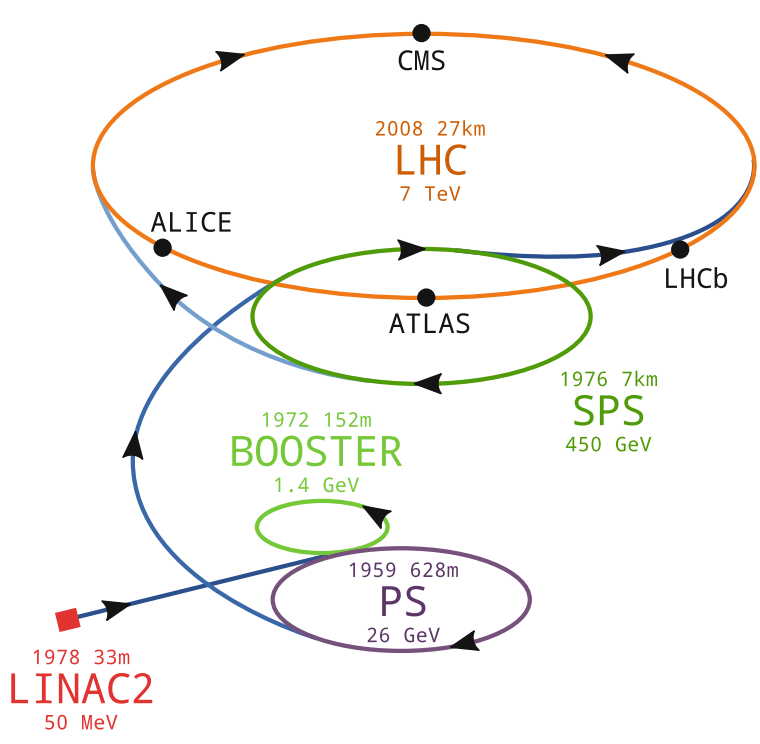
\includegraphics[width=0.6\columnwidth]{./LHCcomplex.png}
  \caption{
    Diagram of the LHC accelerator complex located near Geneva, Switzerland. The complex consists of three accelerator stages: the proton (p) or lead (Pb) source, the Proton Synchrotron (PS), the Super Proton Synchrotron (SPS), and the 27 km LHC ring. Four collision points are shown corresponding to the ALICE, ATLAS, LHCb, and CMS detectors  \cite{Mobs:2684277}.
  }
  \label{figure5}
\end{figure}


\begin{figure}[H]
  \centering
  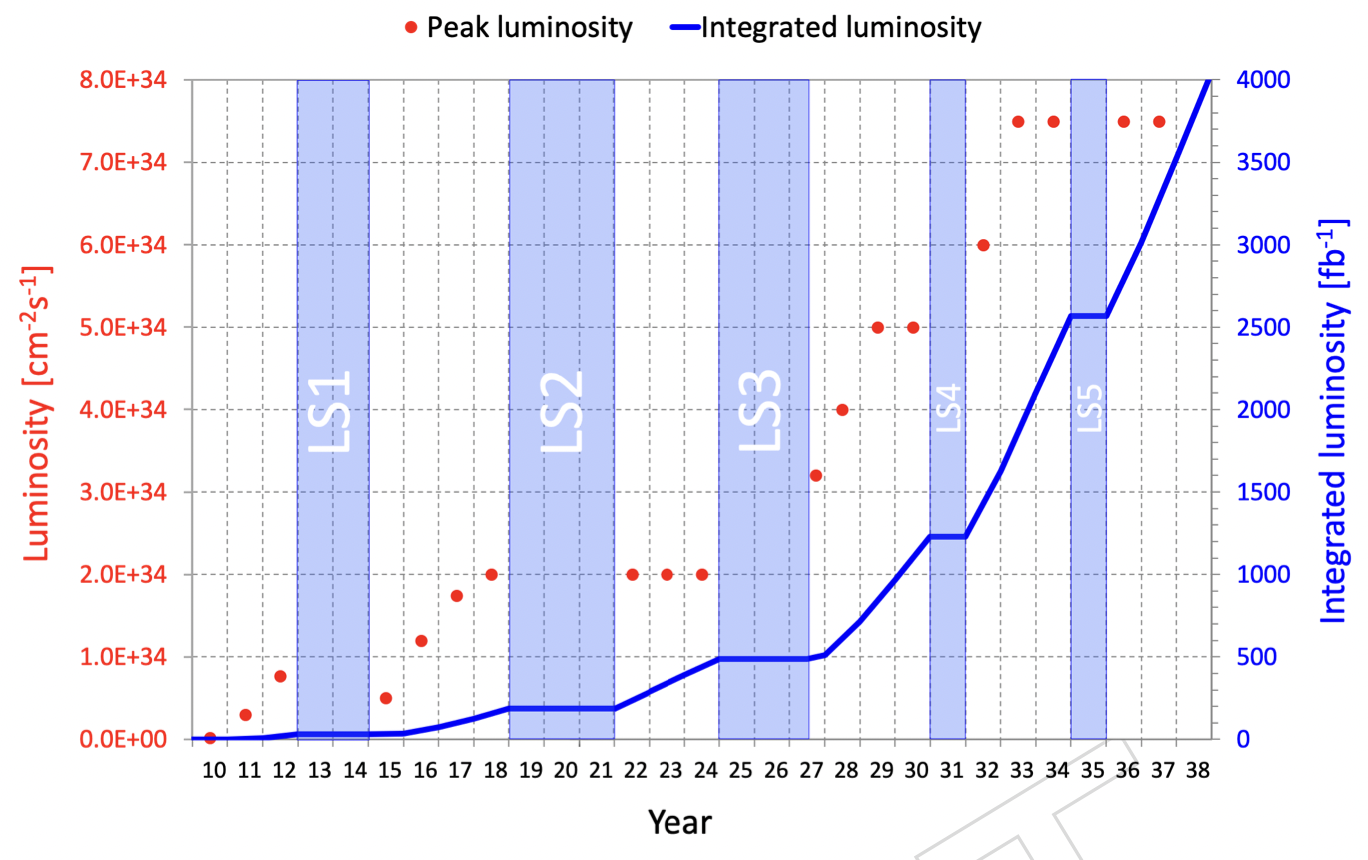
\includegraphics[width=0.8\columnwidth]{./HLLHCLumi.png}
  \caption{
    Projected performance of the LHC until 2038, which shows the preliminary dates for prolonged stops (LS) of the LHC and luminosities. Points show instantaneous luminosity while the line shows luminosity accumulated \cite{collaborations2019report}.
  }
  \label{figure6}
\end{figure}


 \begin{figure}[H]
   \centering
   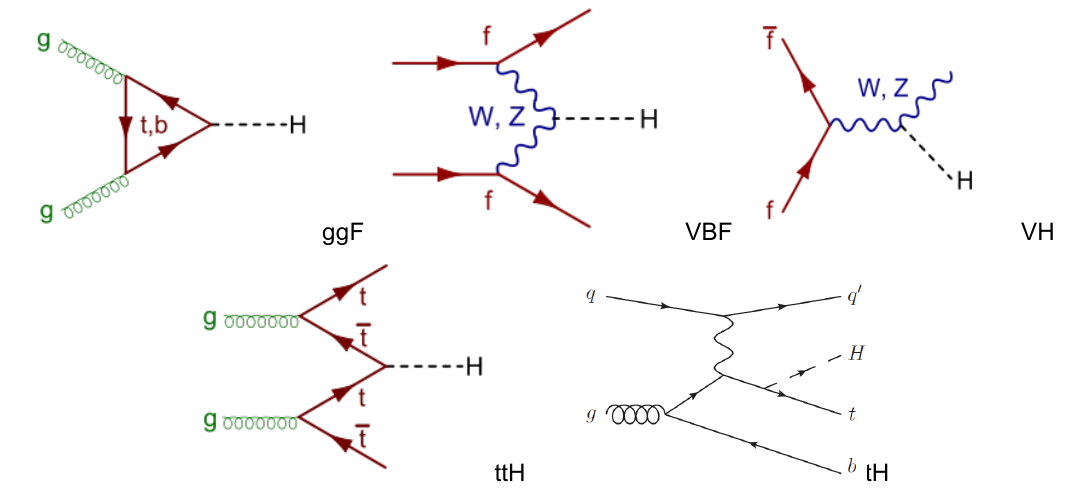
\includegraphics[width=0.7\columnwidth]{./pg.png}
   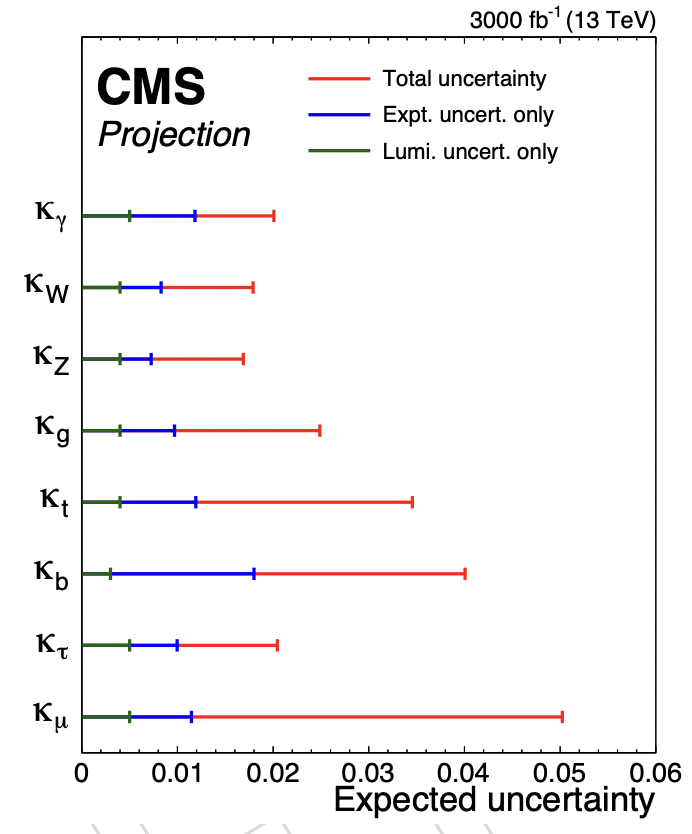
\includegraphics[width=0.29\columnwidth]{./higgs_couplings.png}
   \caption{
     Left: Main production mechanisms for the Higgs boson at the LHC: gluon-gluon fusion (ggF), vector-boson fusion (VBF), associated vector boson (VH), associated top-quark pair (ttH), and  associated single-top quark production (tH)  \cite{Grojean:2017hsb}  \cite{Khachatryan:2015ota} .
     Right: Expected uncertainties on the Higgs coupling parameters for  \lumi{3000} of proton-proton collision data at 13 TeV center-of-mass energy \cite{Cepeda:2019klc}.
   }
   \label{figureKappasUncs}
 \end{figure}




\section{PROPOSAL}

In this project, we aim to make the most precise measurements of the luminosity for the Run 2 (2017-2018) as well as for the Run 3 data taking period (2022-2024).
In addition we expect to perform studies for the design and construction of an upgraded luminosity measurement system to be installed for CMS in the HL-LHC phase \cite{Collaboration:2706512}.


\section{GENERAL OBJECTIVE}

The main objective of this work is to improve on the precision of the preliminary luminosity measurements for the different datasets with the aim to provide a final precision at the level of 1\%.
This precision is needed for the measurement of many important physics processes, like the Higgs boson production crossection, which define the Standard Model of particle physics. 

\section{HYPOTHESIS}

Based on the previous work on the Run 2 (2015-2016) datasets which have achieved a precision at the level of 1.3\%, we expect that a precision at this level or lower will be possible due to the improved methods we are developing.
For reference, the current precision on the Run 2 (2017-2018) and Run 3 (2022) datasets is above 2\%~\cite{Sirunyan:2021qkt}. 



\section{METHODOLOGY}


The CMS experiment is located at one of the four interaction points of the LHC.
The CMS detector has the form of a cylindrical onion, with several concentric layers of components.
A powerful magnet is used to bend charged particles as they move away from the point of collision to identify the charge and measure their momentum.
A silicon tracker, made of about 75 million electronic sensors arranged in concentric layers, measures the curvature of charged particles with very high precision \cite{Chatrchyan:2008aa}.
The electromagnetic calorimeter detects photons and electrons while the hadron calorimeter detects mainly pions and kaons.
The muons are detected by special chambers placed outside the solenoid as shown in Figure~\ref{fig:CMS}.

The PCC method for measuring luminosity uses the Pixel detector of the CMS tracker, the layout of the  detector used for recording the data during 2016-2018 is shown in Figure~\ref{fig:pixeldet},  this detector is expected to deliver high-quality data until the end of LHC Run 3 (currently expected for 2024).
The Pixel detector consists of 4 concentric cylindrical layers in the barrel and 3 disks in each endcap.
Each detector part is composed of pixel sensors, a schematic of one sensor is shown in Figure~\ref{fig:pixeldet}.
The entire Pixel detector contains 1856 sensor modules and a total of 124 million pixels \cite{TrackerGroupoftheCMS:2020bgg}.

The PCC method consists of the reconstruction of track clusters produced by charged particle tracks as shown in Figure~\ref{fig:bunchcrossing}.
Due to the fine granularity of the pixel sensors and the large number of total pixels, the hit occupancy in the sensors remains very small, order of 1\%, during normal collisions.
This low occupancy makes the PCC  very linear as a function of pileup, an essential property of a good luminometer \cite{Sirunyan:2021qkt}.

The calibration of the luminometer consists of a van der Meer (vdM) scan performed in a special LHC run usually at the beginning of the run period (year).
These scans are performed by varying the separation between the beams in each direction ($x$ and $y$) at a fixed number of separation steps of about 100 micrometers. Then these rates are fitted by a Gaussian function to obtain the beam overlaps $\Sigma_{x,y}$ and the peak rate of clusters $R(0,0)$ \cite{CMS:2018}. A schematic view of this methos is shown in Fig. \ref{vdMSketch}. 
Finally the calibration constant ($\sigma_{vis}$) is determined as Eq.\ref{sigmavis_eq}.

\begin{equation}
  \sigma_{vis}=\frac{2\pi \Sigma_{x} \Sigma_{y} R(0, 0)}{N_{1}N_{2} f}
  \label{sigmavis_eq}
\end{equation}
Where $f$  is the LHC frecuency and $N_{1},N_{2}$ are the buch current used to normalize  the rates.
This calibration constant is then used to determine the luminosity during a normal running throughout the data-taking year \cite{CMS:2018}.

For the upgrade part of this project, the research consists of studying the expected performance of the TEPX disks of the CMS tracker in the HL-LHC phase.
The current design of the this tracker is shown in Figure~\ref{fig:tepx}, where the TEPX part consists of the last 4 disks at $|z|>170$ cm. In the same figure a transverse view of one disk is shown, and shows the layout of the sensor modules along phi for each ring in the disk \cite{Klein:2017nke}.
Studies will be performed using simulated samples with HL-LHC beam conditions, currently the expected pileup for these conditions is about 200 proton collisions per bunch crossing.
The linearity of the cluster counting algorithm will be studied.
In addition, a new algorithm may be developed to detect cluster coincidences between consecutive layers of a disk.
%It is expected that coincidences will be less sensitive to backgrounds in HL-LHC pileup conditions and therefore a more robust luminosity measurement can be performed.


\begin{figure}[H]
  \centering
  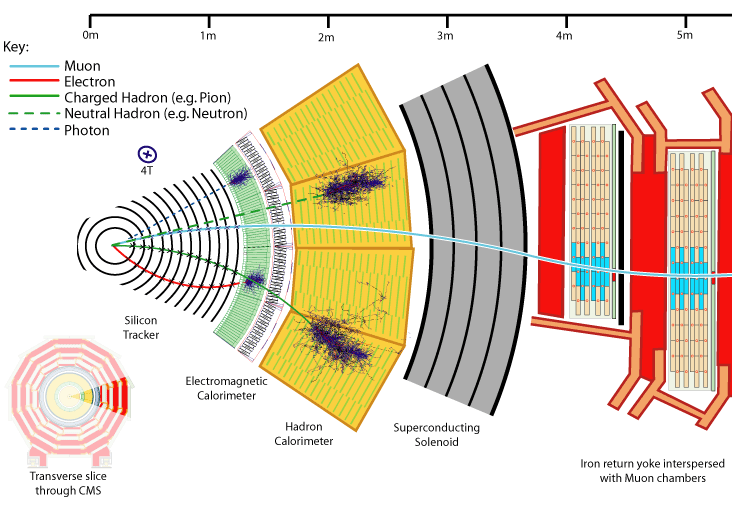
\includegraphics[width=0.65\columnwidth]{./cms12.png}
  \caption{Transverse view of the CMS detector showing the silicon tracker, electromagnetic calorimeter, hadron calorimeter, superconducting solenoid and muon chambers \cite{Chatrchyan:2008aa}.}
  \label{fig:CMS}
\end{figure}


\begin{figure}[H]
  \centering
  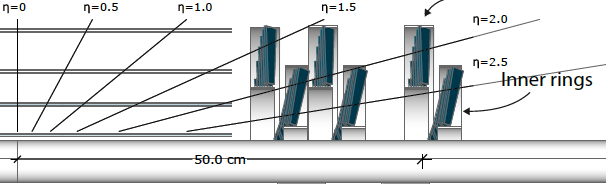
\includegraphics[width=0.7\columnwidth]{./PixelDetectorPhase1.png}
  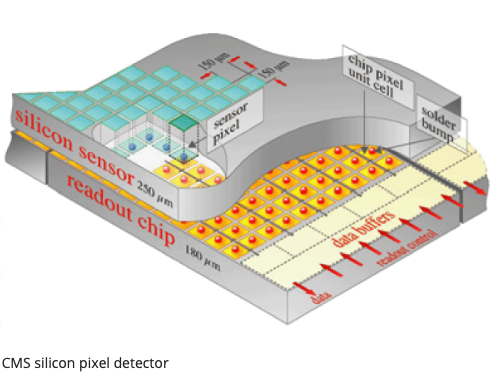
\includegraphics[width=0.27\columnwidth]{./PixelSensor.png}
  \caption{
    Left: diagram showing the layout of the CMS Pixel detector used during 2016-2018.
    The layout consists of 4 barrel layers and 2 endcap disks with two rings each.
    Right: a diagram showing the structure of one pixel sensor.
    The entire detector consists of 1856 sensors and 65 million pixels \cite{TrackerGroupoftheCMS:2020bgg}.
  }
  \label{fig:pixeldet}
\end{figure}

\begin{figure}[H]
  \centering
  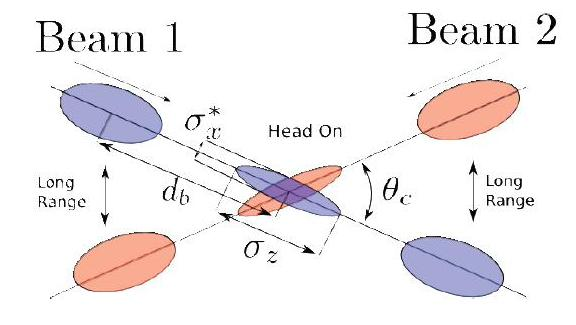
\includegraphics[width=0.48\columnwidth]{./bunchcrossing.jpg}
  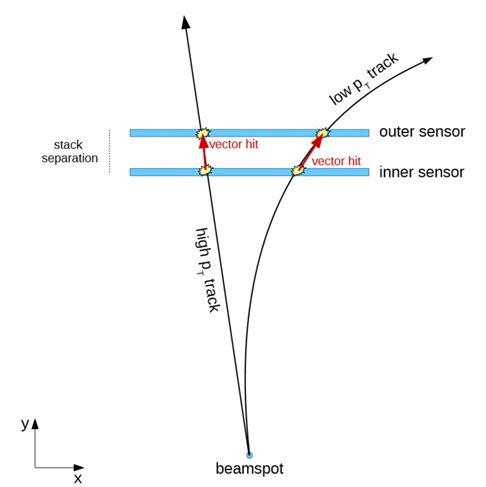
\includegraphics[width=0.48\columnwidth]{./vectorhit1.jpg}
  \caption{
    Left: Dagram showing the collision of two proton bunches at LHC, bunches contain about $10^{11}$ protons  \cite{deMaria:2008zzb}.
    Right: diagram showing example tracks originating from the collision and producing hits in the pixel detector layers.
  }
  \label{fig:bunchcrossing}
\end{figure}


\begin{figure}[H]
  \centering
  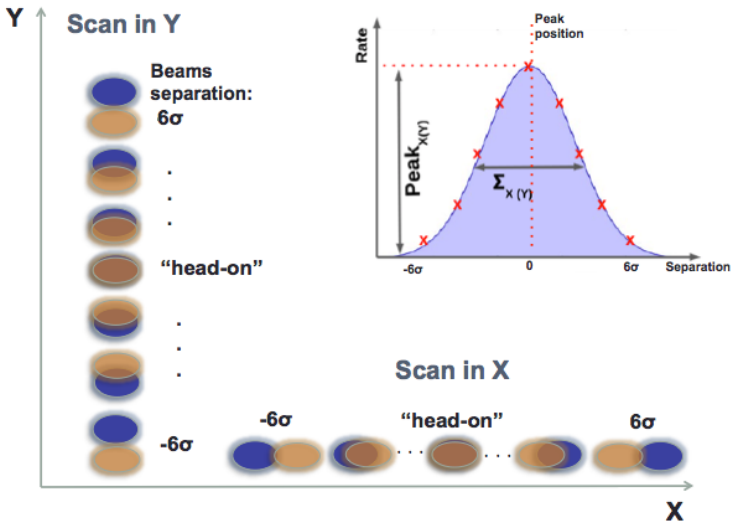
\includegraphics[width=0.7\columnwidth]{./vdm_sketch.png}
  \caption{
   Sketch of a vdM scan in x and y planes. The sketch is an example of
the fit of the resulting cluster rates \cite{vdMSketch}.
  }
  \label{vdMSketch}
\end{figure}

\begin{figure}[H]
  \centering
  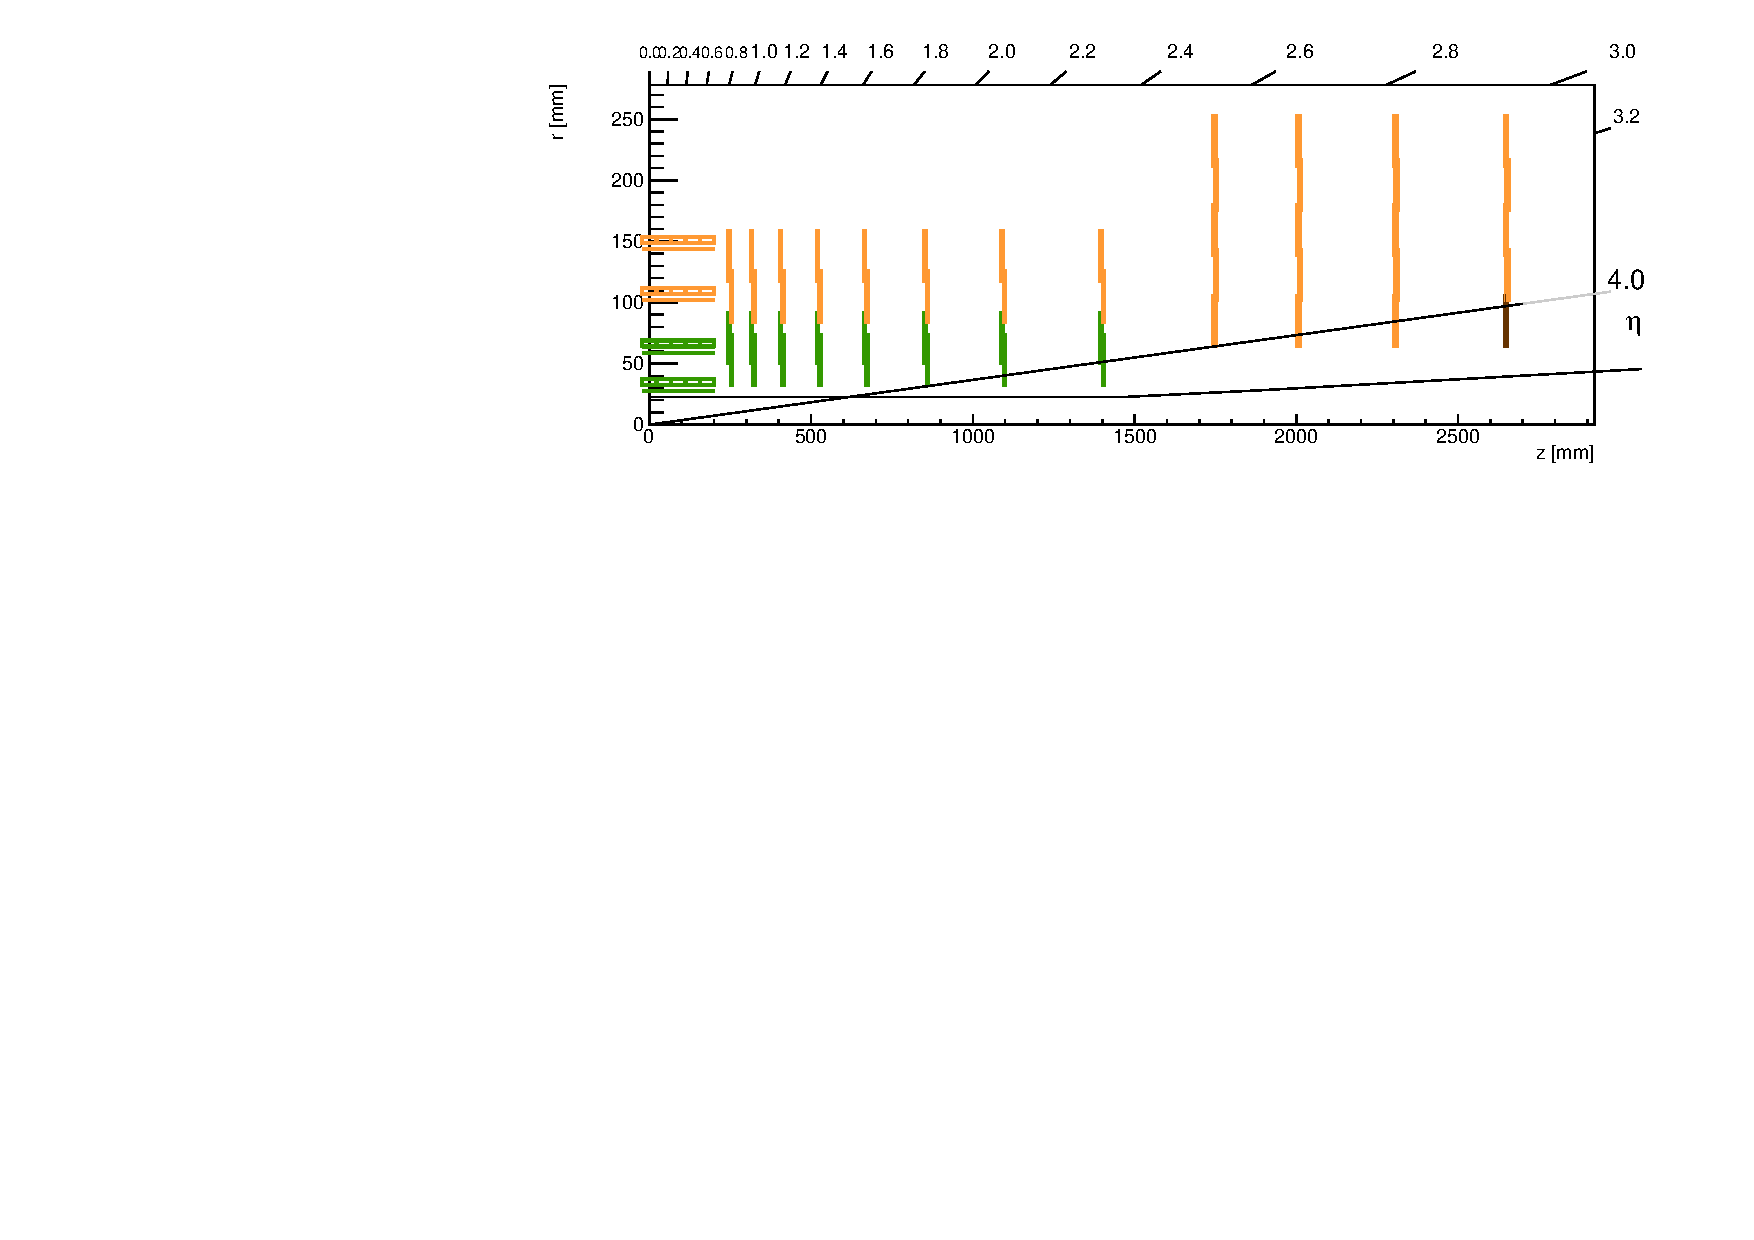
\includegraphics[width=0.7\columnwidth]{./TEPX_rz.pdf}
  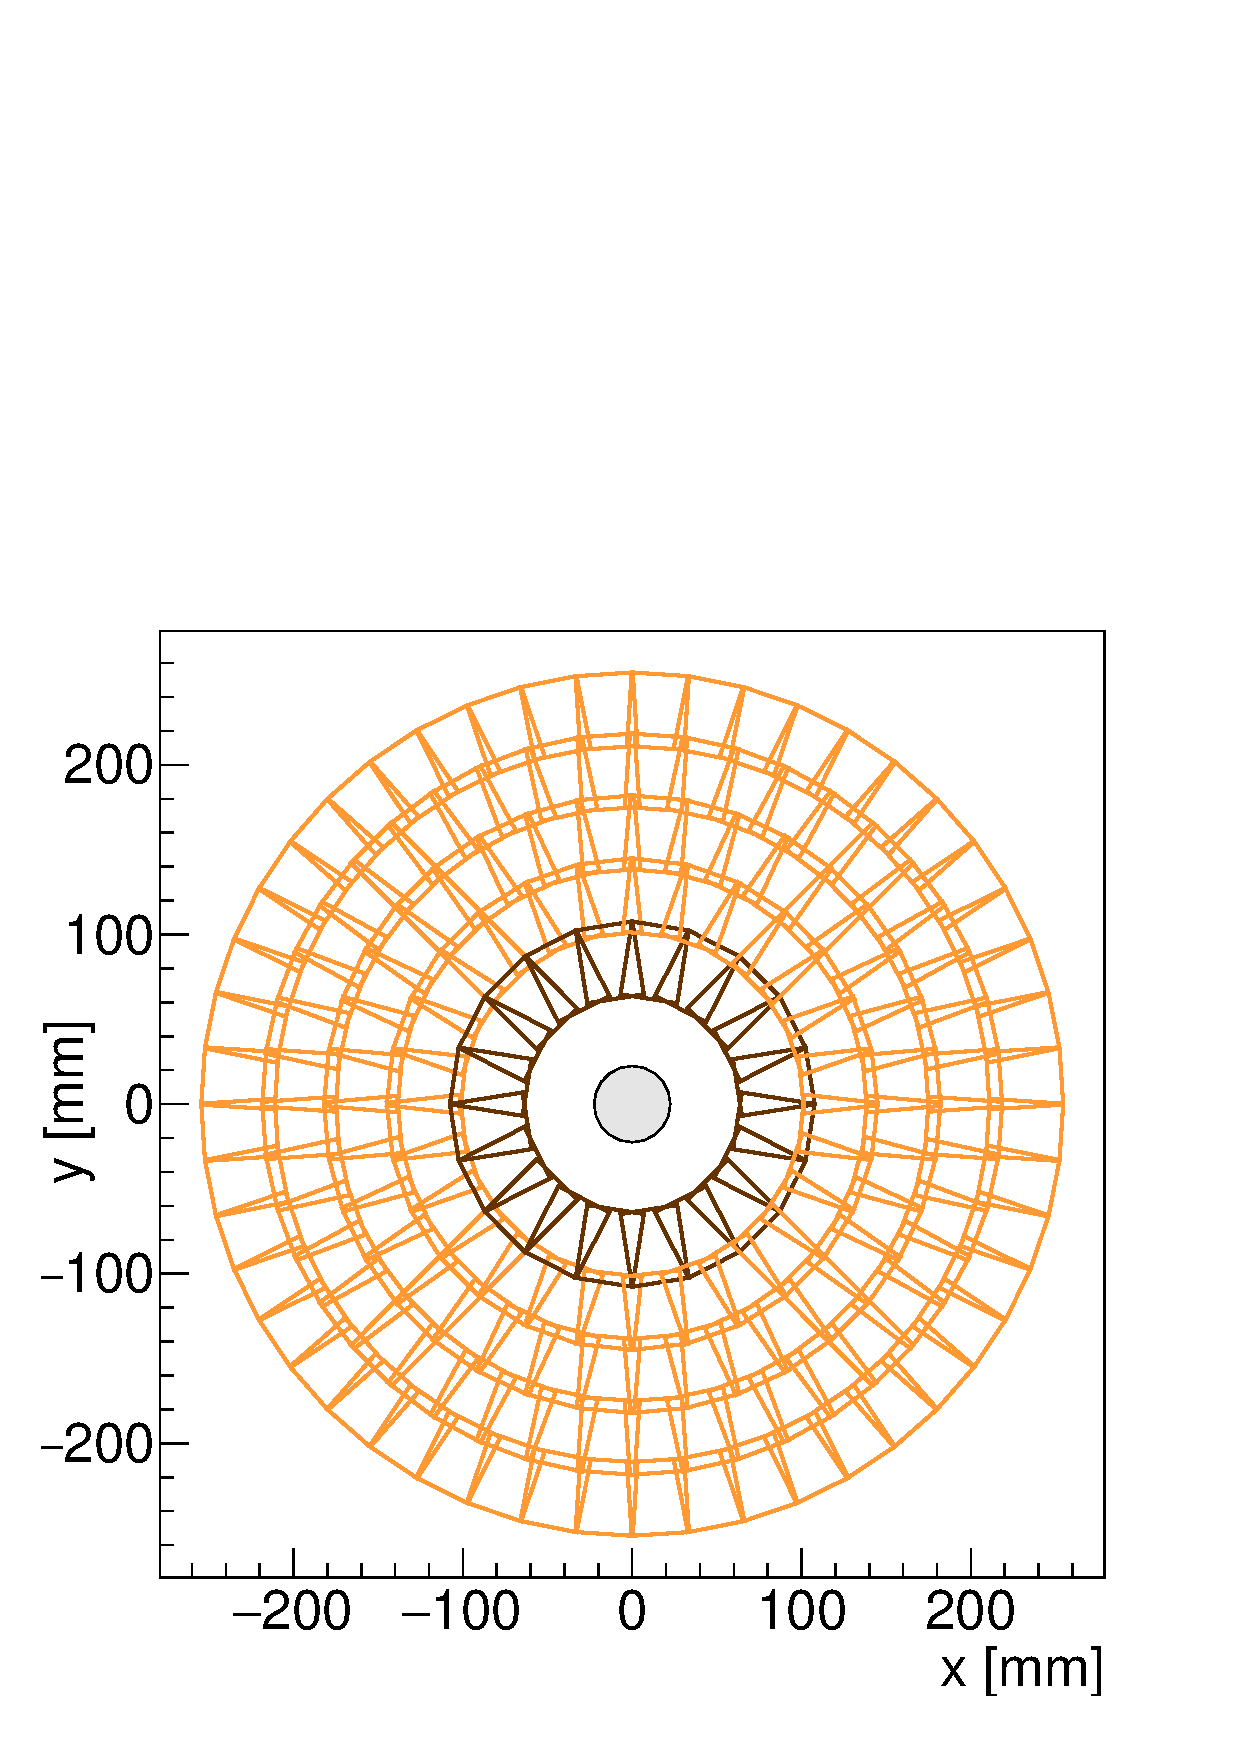
\includegraphics[width=0.27\columnwidth]{./TEPX_rphi.pdf}
  \caption{
    Left: Longitudial view of the current design of the CMS tracker detector for the HL-LHC phase. The TEPX consists of the last 4 disks on each side at $|z|>$ 1700 mm.
    Right: Transverse view of one TEPX disk showing the layout of the sensors in each of the 5 rings \cite{Klein:2017nke}.
  }
  \label{fig:tepx}
\end{figure}



\section{SPECIFIC OBJECTIVES}

For the Run 2 and Run 3 luminosity measurements:
\begin{itemize}
\item Understand the CMS pixel detector layout including the barrel layers and endcap disks and their constituent modules.
\item Study the stability of the modules in the different layers or disks of the pixel detector and select the stable components.
\item Calculate the calibration constant (visible crossection) corresponding to 13.6 TeV proton-proton collision data.
\item Study the stability and linearity of the PCC luminosity measurement by comparing to other CMS luminometers.
\item Determine the instantaneous and the total integrated luminosity.
\item Determine the systematic uncertainties on the calibration constant and on the integrated luminosity.
\end{itemize}

\par
For the development of the HL-LHC upgrade system:
\begin{itemize}
\item Study the different parts of the TEPX detector.
\item Study the pixel cluster counting at the HL-LHC conditions using simulations of the TEPX detector.
\item Develop algorithms for pixel  cluster counting and coincidence counting.
\item determine the linearity and  precision of the different methods.
\end{itemize}


\section{EXPECTED RESULTS}

From this project two main publications are expected:
\begin{itemize}
\item For the Run 2 luminosity mesurement, studies of the selection of good detector modules, calibration, background estimation, and calculation of the integrated luminosity, including the systematic uncertainties will be completed.
The results of these studies will be published in a peer-reviewed scientific journal.
\item For the Run 3 luminosity measurement, no measurement of the luminosity precision has been performed at this moment.
Similar studies as for the Run 2 dataset will be performed completed and a preliminary result of the luminosity measurement will be published.
\item For the development of the HL-LHC upgrade system, the work  will be based on the previously published Technical Design Report (TDR) with the proposed design and algorithms to use the TEPX detector.
It is expected that this work will be presented at conferences and used for the final design and construction of the system to be installed in the LS3 (2025-2027).  
\end{itemize}

Also, the student will become a part of an international experiment and is expected to present his results at national or international scientific conferences.



\section{CALENDAR OF ACTIVITIES}

\begin{itemize}

\item {\bf Semester 1 (2023-2)}:
  \SubItem{ Readings on Standard Model of physics theory, LHC, and CMS experiments.}
  \SubItem{ Review of the literature.}
  \SubItem{ Master Linux computing and data analysis  skills (\textsc{Bash, Emacs, Root, HTCondor parallel processing.})}
  \SubItem{ Complete work on the 2022 luminosity measurement for a preliminary  publication.}

\item {\bf Semester 2 (2024-1)}:
  \SubItem{ Course I on particle physics, particle detection, or data analysis.}
  \SubItem{ Continue readings on Standard Model of physics theory, LHC, and CMS experiments.}
  \SubItem{ Master Linux computing and data analysis  skills (\textsc{Bash, Emacs, Root, HTCondor parallel processing.})}
  \SubItem{ Complete work on the Run 2 luminosity measurement for a final  publication.}
  \SubItem{ Start work on the 2023 dataset luminosity measurement. }
  
\item {\bf Semester 3 (2024-2)}:
  \SubItem{ Course II on particle physics, particle detection, or  data analysis.}
  \SubItem{ Complete work on the 2023 dataset luminosity measurement.}
  \SubItem{ Start work on the 2024 dataset luminosity measurement. }
  
\item {\bf Semester 4 (2025-1)}:
  \SubItem{ Continue work on the 2024 dataset luminosity measurement. }
  \SubItem{ Start studies on the TEPX luminometer for the HL-LHC.}
  \SubItem{ Writing of the monograph.}

\item {\bf Semester 5 (2025-2)}:
  \SubItem{ Complete work on the 2024 dataset luminosity measurement. }
  \SubItem{ Complete studies on the TEPX luminometer for the HL-LHC.}
  \SubItem{ Presentation at national or international conferences of the TEPX upgrade studies.}
  
\item {\bf Semester 6 (2026-1)}:
  \SubItem{ Start final studies of the Run 3 data luminosity measurement for publication in a peer reviewed journal.}

\item {\bf Semester 7 (2026-2)}:
  \SubItem{ Completion of the studies of the Run 3 data luminosity measurement for publication in a peer reviewed journal.}
  \SubItem{ Presentations at national or international conferences of the luminosity measurements and TEPX luminometer for HL-LHC.}
  \SubItem{ Writing of the Ph.D thesis.}
  
\item {\bf Semester 8 (2027-1)}: 
  \SubItem{ Publication of the Run 3 data luminosity measurement in a peer reviewed journal.}
  \SubItem{ Presentations at national or international conferences of the luminosity measurements and TEPX luminometer for HL-LHC.}
  \SubItem{ Defense of the Ph.D thesis.}
  
\end{itemize}


\onehalfspacing
\bibliographystyle{unsrt}
\bibliography{paper}

\end{document}

